\documentclass[12pt,a4paper]{article}
%\usepackage[cp1251]{inputenc}
\usepackage[utf8]{inputenc}
\usepackage[T2A]{fontenc}
\usepackage[english,russian]{babel}
\usepackage{amscd,amssymb}
\usepackage{amsfonts,amsmath,array}
\usepackage[dvips]{graphicx}
\usepackage{longtable,wrapfig}
\usepackage{pstricks}
\usepackage{ifpdf}
\usepackage{amsmath}
\newtheorem{theorem}{Теорема}

\textheight= 25cm \textwidth= 16cm \hoffset= -1.cm
\voffset= -2.4cm

\begin{document}

\renewcommand\refname{\centering \textit{\small{Литература}}}

\begin{center}
{\large\bf Методы PCA и SVD} \\[5mm] Р.\,М.~Селевенко \\
 Московский Государственный Университет, Факультет ВМК\\
\end{center}

При обработке больших массивов данных представленных в виде таблицы объектов и признаков  возникает потребность в обработке этой таблицы с целью упрощения структуры данных.
А именно, выделения объектов представляющих собой частные случае вместо части общей выборки. А также выделения признаков представляющих собой линейную комбинацию других признаков. 
Например, в случае предсказания цены на комнаты в гостинице, нам могут быть даны такие фичи как площадь комнаты, длина и ширина периметра комнаты.
В этом случае фичи длины и ширины нам не нужны т.к. они являются простой линейной комбинацией площади. 
Также существует так называемое "проклятие размерности" - при увеличении размерности простравнства количество данных возростает экспоненциально.

\begin{figure}[h]
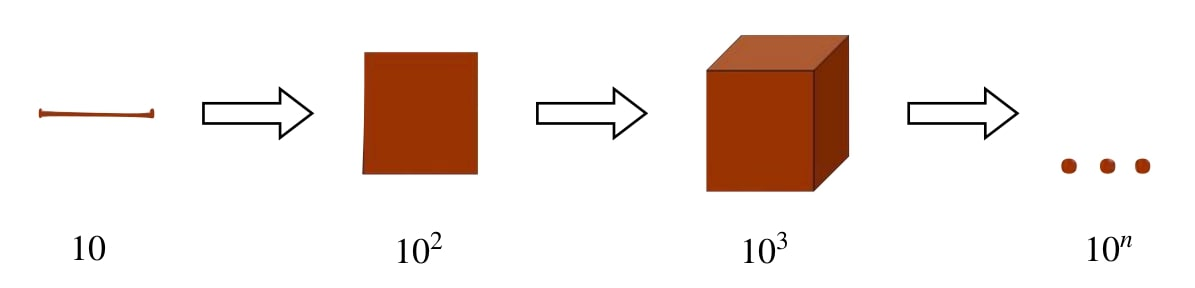
\includegraphics[scale=0.75, width = 480, height = 100]{dimension.jpg}
\caption{Пример проклятия размерности.}
\label{ris:image}
\end{figure}

Для устранения этой проблемы можно выбросить часть признаков или построить меньшее количество признаков на основе старых.

Цель: построить	меньшее количество новых признаков, которые содержат максимум информации из исходных.
Для начала рассмотрим Principal Component Analysis (PCA), метод главных компонент.
Пусть есть матрица $F_{l,n}$ где $l$ - количество объектов, $n$ - количество признаков.
Хотим сократить количество признаков с n до m. 
При этом старые признаки должны как можно точнее линейно восстанавливаться по новым на обучающей выборке.

$$
    f_j^{*}(x) = \sum_{s=1}^{m}g_s(x)u_{js}, j=1, \ldots, n, \forall x \in X
$$

Старые признаки $f_j$ - линейная комбинация новых $g_s$.

Хотим восстанавливать старые признаки из новых, как можно точнее:

$$
    \sum_{i=1}^{l}\sum_{j=1}^{n}(f_j^{*}(x_i) - f_j(x_i))^2 \rightarrow \min\limits_{\{g_s(x_i)\}, \{u_{js}\}}
$$

Матрицы объекты признаки:

\[
F_{l * n}
=
\begin{bmatrix}
    f_1(x_1) & \dots  & f_n(x_1) \\
    \vdots & \vdots & \vdots \\
    f_1(x_l) & \dots  & f_n(x_l)
\end{bmatrix}
\]

\[
G_{l * m}
=
\begin{bmatrix}
    g_1(x_1) & \dots  & g_m(x_1) \\
    \vdots & \vdots & \vdots \\
    g_1(x_l) & \dots  & g_m(x_l)
\end{bmatrix}
\]

Матрица линейного преобразования новых признаков в старые:

\[
U_{n * m}
=
\begin{bmatrix}
    u_{11} & \dots  & u_{1m} \\
    \vdots & \vdots & \vdots \\
    u_{n1} & \dots  & u_{nm}
\end{bmatrix}
\]

$$
    F^* = GU^T
$$

Мы хотим чтобы:

$$
    F^* = F
$$

Из этого имеем:

$$
    \| GU^{T} - F \|^2 \rightarrow \min\limits_{G, U}
$$

\begin{theorem} \label{t1} 
    Если $m <= rkF$, то минимум $\| GU^T - F\|^2$ достигается, когда столбцы $U$ - это с.в. матрицы $F^TF$, соответствующие $m$ максимальным с.з. $\lambda_1, \ldots, \lambda_m$, а матрица $G=FU$.
    При этом:
    \\1. матрица $U$ ортонормирована: $U^TU=I_m$;\\
    2. матрица $G$ ортогональна: $G^TG=\Lambda=diag(\lambda_1, \ldots, \lambda_m)$;\\
    3. $U\Lambda=F^TFU$;$G\Lambda=FF^TG$;\\
    4. $\|GU^T - F\|^2 = \|F\|^2 - tr\Lambda = \sum_{j=1}^{n}\lambda_j - \sum_{j=1}^{m}\lambda_j=\sum_{j=m+1}^{n}\lambda_j$;\\
\end{theorem}

Матрица $G$ ортогональна $G^TG = \Lambda = diag(\lambda_1, \ldots, \lambda_m)$ а значит, новые признаки образуют базис.

\begin{figure}[h]
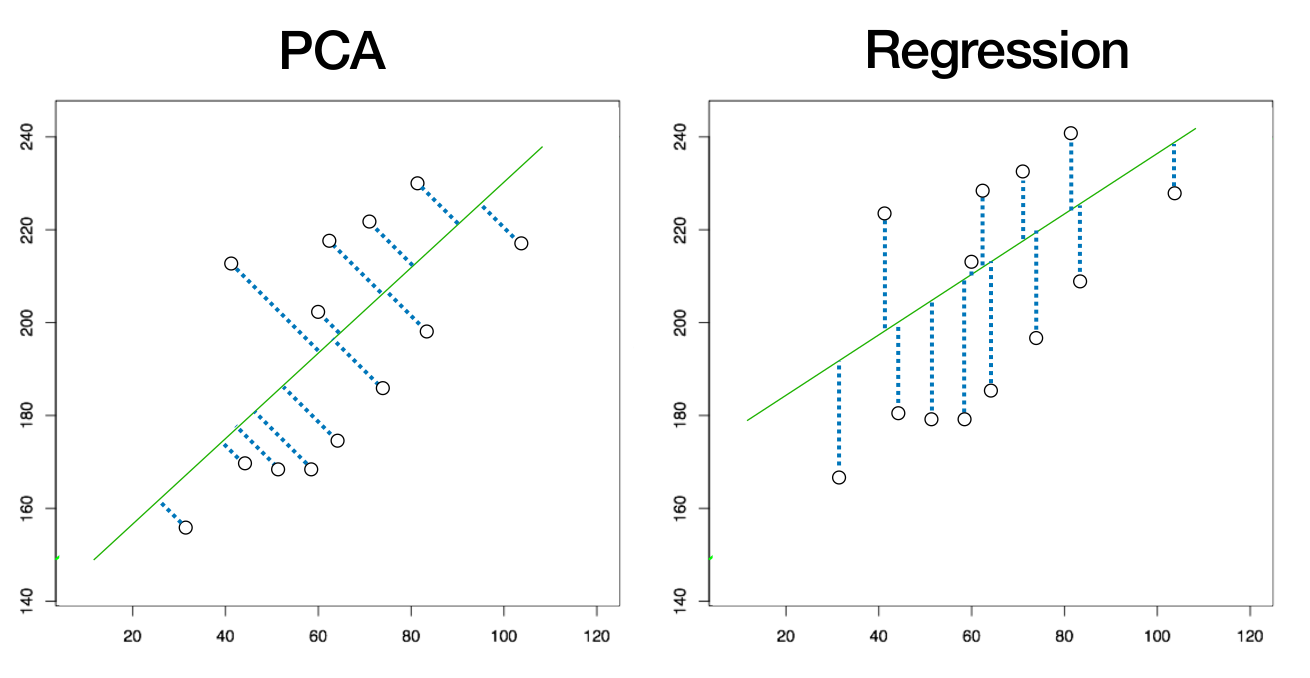
\includegraphics[scale=0.75, width = 480, height = 200]{regression.png}
\caption{Пример работы линейной регрессии и PCA.}
\label{ris:image}
\end{figure}

Обобщая, PCA ищет такую гиперплоскость, суммарное расстояние от точек выборки до которых будет минимально.
PCA ищет такие ортогональные проекции, дисперсия вдоль которых для точек выборки будет максимальна.
PCA строит такой базис, в котором новые признаки ортогональны.\\

Допустим что мы построили такую плоскость. Как выбрать количество новых признаков?
Собственные числа упорядочены по убыванию:

\begin{figure}[h]
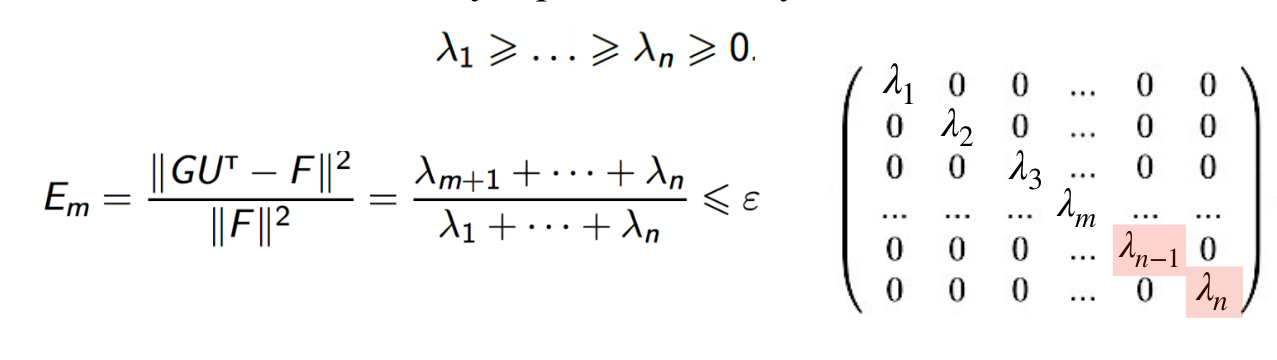
\includegraphics[scale=0.75, width = 400, height = 150]{sz.png}
\label{ris:image}
\end{figure}

\begin{figure}[h]
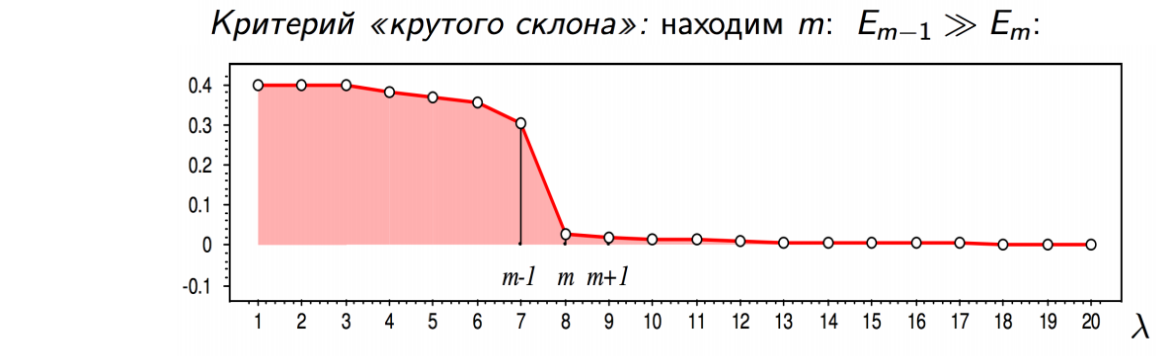
\includegraphics[scale=0.75, width = 480, height = 200]{krutoi_sklon.png}
\label{ris:image}
\end{figure}

Здесь видно, что есть некое значение $m$, такое что $E_m$ намного меньше чем $E_{m-1}$ именно это значение и будет количеством признаков, которые должны остаться в нашей таблице.

Теперь рассмотрим метод SVD (Singular Value Decomposition).\\
Он основан на утверждении, что:
$$
    F_{l, n} = V_{l, n} * \Sigma_{n, n} * U^T_{n, n}
$$
, где $V$ и $U$ - ортоганальные матрицы (состоят из левых и правых сингулярных векторов), $\Sigma$ - на главной диагонали сингулярные числа.\\
\\
\\
\\
\\
\\


\begin{figure}[h]
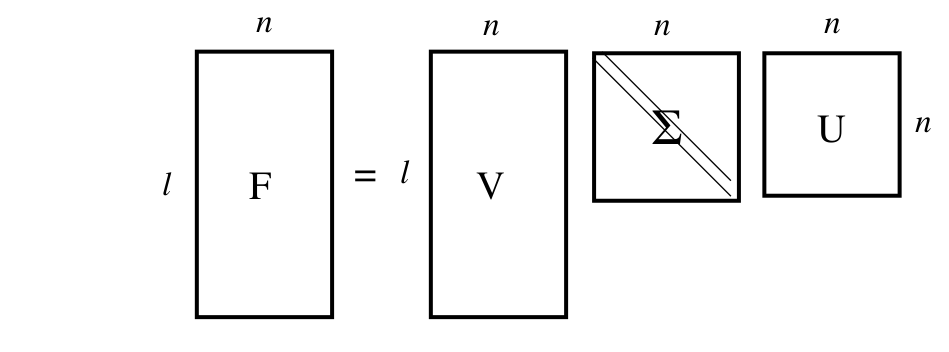
\includegraphics[scale=0.75, width = 480, height = 200]{singular_value_decomp.png}
\caption{Размеры матриц в SVD разложении.}
\label{ris:image}
\end{figure}

Пусть исходная матрица $F$ задает некоторое линейное преобразование исходного пространства. 
Тогда линейное преобразование можно рахбить на последовательность более простых преобрахований.

\begin{figure}[h]
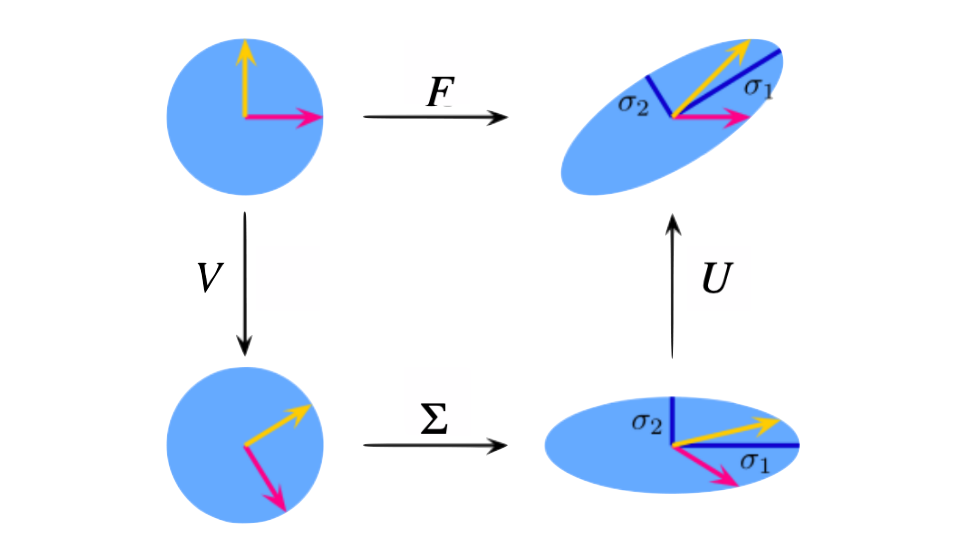
\includegraphics[scale=0.75, width = 480, height = 200]{Screenshot from 2022-10-22 22-07-19.png}
\label{ris:image}
\end{figure}

Можно взять $m$ строк матрицы $\Sigma$, соответствующие наибольшим сингулярным числам, m столбцов матриц $V$ и $U$ $\rightarrow$ получить приближенное представление матрицы $F$.
$$
    F^{*}_{l, n} = V_{l, m} * \Sigma_{m, m} * U^T_{m, n}
$$

\begin{figure}[h]
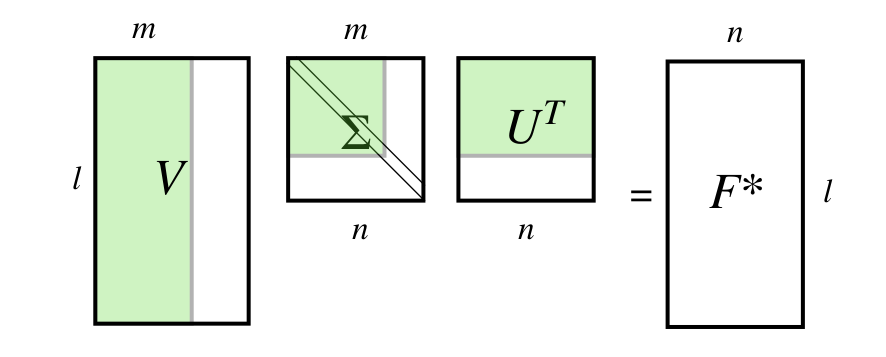
\includegraphics[scale=0.75, width = 240, height = 100]{truncated.png}
\label{ris:image}
\end{figure}

Сравним PCA и SVD.

PCA:\\
$$
    F_{l, m} = G_{l, m} * U^T_{m, n}
$$

SVD:\\
$$
    F^{*}_{l, n} = V_{l, m} * \Sigma_{m, m} * U^T_{m, n}
$$

В качестве новых признаков можно взять произведение первых двух матриц:

$$
    G_{l, m} = V_{l, m} * \Sigma_{m, m}
$$

\begin{figure}[h]
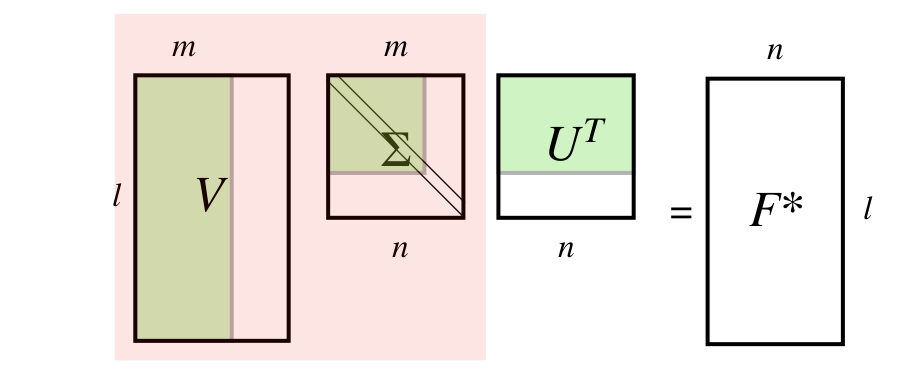
\includegraphics[scale=0.75, width = 240, height = 100]{choose.png}
\label{ris:image}
\end{figure}

\end{document} 